\chapter{Results \& Discussion}\label{chap:results}

In this chapter, the results of the experiments are presented and discussed. The experiments were conducted to evaluate the impact of different neural network structures and parameters on image reconstruction. The experiments were conducted using the four neural network architectures described in Chapter \ref{chap:experiments}. The neural networks were trained and tested using the datasets described in Section \ref{sec:datasets}. The experiments were conducted using the training and testing procedures described in Section \ref{sec:Experimental procedures}.

\section{Graph parameters}

The graph parameters calculated in the experiments are shown in Table \ref{tab:gp1}~\ref{tab:gp2}. 

\section{Graph Convolutional Networks}
The calculated generalization error of the experiments using Graph Convolutional Networks are shown in Table~\ref{tab:ge_gcn}.


\begin{table}[!ht]
    \centering
    \footnotesize
    \begin{tabular}{p{3.5cm}|p{5cm}p{5cm}}
    \hline
    \toprule
        Name & Ave. generalization error & Standard deviation \\ 
    \midrule
        AIDS & 0.0081874905154109 & 0.0117165874689817 \\ 
        BZR & 0.0708846226334571 & 0.0609733723104 \\ 
        BZR\_MD & 0.0961788743734359 & 0.1091229766607284 \\ 
        COLORS-3 & 0.06828124076128 & 0.0298492461442947 \\ 
        COX2 & 0.0840000063180923 & 0.1163316890597343 \\ 
        COX2\_MD & 0.0750205665826797 & 0.1105385944247245 \\ 
        DD & 0.0138164404779672 & 0.0569455623626709 \\ 
        DHFR & 0.1413267403841018 & 0.0572429783642292 \\ 
        DHFR\_MD & 0.0547252781689167 & 0.1071747243404388 \\ 
        ENZYMES & 0.1968750059604644 & 0.1035036742687225 \\ 
        ER\_MD & 0.0477907545864582 & 0.0669434815645217 \\ 
        FRANKENSTEIN & 0.0549374930560588 & 0.0326129123568534 \\ 
        KKI & 0.1822761297225952 & 0.3100946843624115 \\ 
        MCF-7 & 0.0019999979995191 & 0.0135001158341765 \\ 
        MCF-7H & 0.003406238509342 & 0.0127300517633557 \\ 
        MOLT-4 & 0.0015624940861016 & 0.0123682264238595 \\ 
        MOLT-4H & 0.0034062266349792 & 0.0167727246880531 \\ 
        MUTAG & 0.1002193242311477 & 0.0946124866604805 \\ 
        Mutagenicity & 0.040156252682209 & 0.0229900479316711 \\ 
        NCI-H23 & 0.0028750181663781 & 0.0120867453515529 \\ 
        NCI-H23H & 0.0005312621360644 & 0.0108473878353834 \\ 
        NCI1 & 0.0832187384366989 & 0.0319501645863056 \\ 
        NCI109 & 0.0711562559008598 & 0.0383276790380477 \\ 
        OHSU & 0.3857143521308899 & 0.2356772273778915 \\ 
        OVCAR-8 & 0.0038125098217278 & 0.0155245345085859 \\ 
        OVCAR-8H & 0.0028437494765967 & 0.0162141937762498 \\ 
        P388 & 0.0043125031515955 & 0.013600654900074 \\ 
        P388H & 0.0070000053383409 & 0.0142645183950662 \\ 
        PC-3 & 0.0024375021457672 & 0.0098565947264432 \\ 
        PC-3H & 0.0060312449932098 & 0.0117860734462738 \\ 
        PROTEINS\_full & 0.0026662945747375 & 0.0525967963039875 \\ 
        PTC\_FM & 0.0923068895936012 & 0.1087017878890037 \\ 
        PTC\_FR & 0.1018810272216796 & 0.1225867569446563 \\ 
        PTC\_MM & 0.088215485215187 & 0.0875236690044403 \\ 
        PTC\_MR & 0.0782608613371849 & 0.0882423818111419 \\ 
        Peking\_1 & 0.2760869860649109 & 0.2045421004295349 \\ 
        SF-295 & 0.0032500028610229 & 0.0157351642847061 \\ 
        SF-295H & 0.0017812550067901 & 0.0091287596151232 \\ 
        SN12C & 0.0003750085888896 & 0.0128499586135149 \\ 
        SN12CH & 0.0031250000465661 & 0.0179813411086797 \\ 
        SW-620 & 0.0014062583213672 & 0.0130064394325017 \\ 
        SW-620H & 0.0014687419170513 & 0.0133227882906794 \\ 
        SYNTHETIC & 0.0120833460241556 & 0.0160114392638206 \\ 
        SYNTHETICnew & 0.1366666555404663 & 0.1849549412727356 \\ 
        Synthie & 0.1234375014901161 & 0.0413857623934745 \\ 
        UACC257 & 0.0011249959934502 & 0.0108615579083561 \\ 
        UACC257H & 0.000843757414259 & 0.0126192783936858 \\ 
        Yeast & 0.0053749978542327 & 0.027795847505331 \\ 
        YeastH & 0.0001875102461781 & 0.0135009009391069 \\ 
    \end{tabular}
    \caption{Generalization error of the GCN model on 49 datasets}
    \label{tab:ge_gcn} % ge -> generalization error
\end{table}

The correlation between the generalization error and the graph parameters are shown in Figure~\ref{fig:correlation_GCN} and Figure~\ref{fig:correlation_ignore_less_than_1000_GCN}.

\begin{figure}[H]
    \centering
    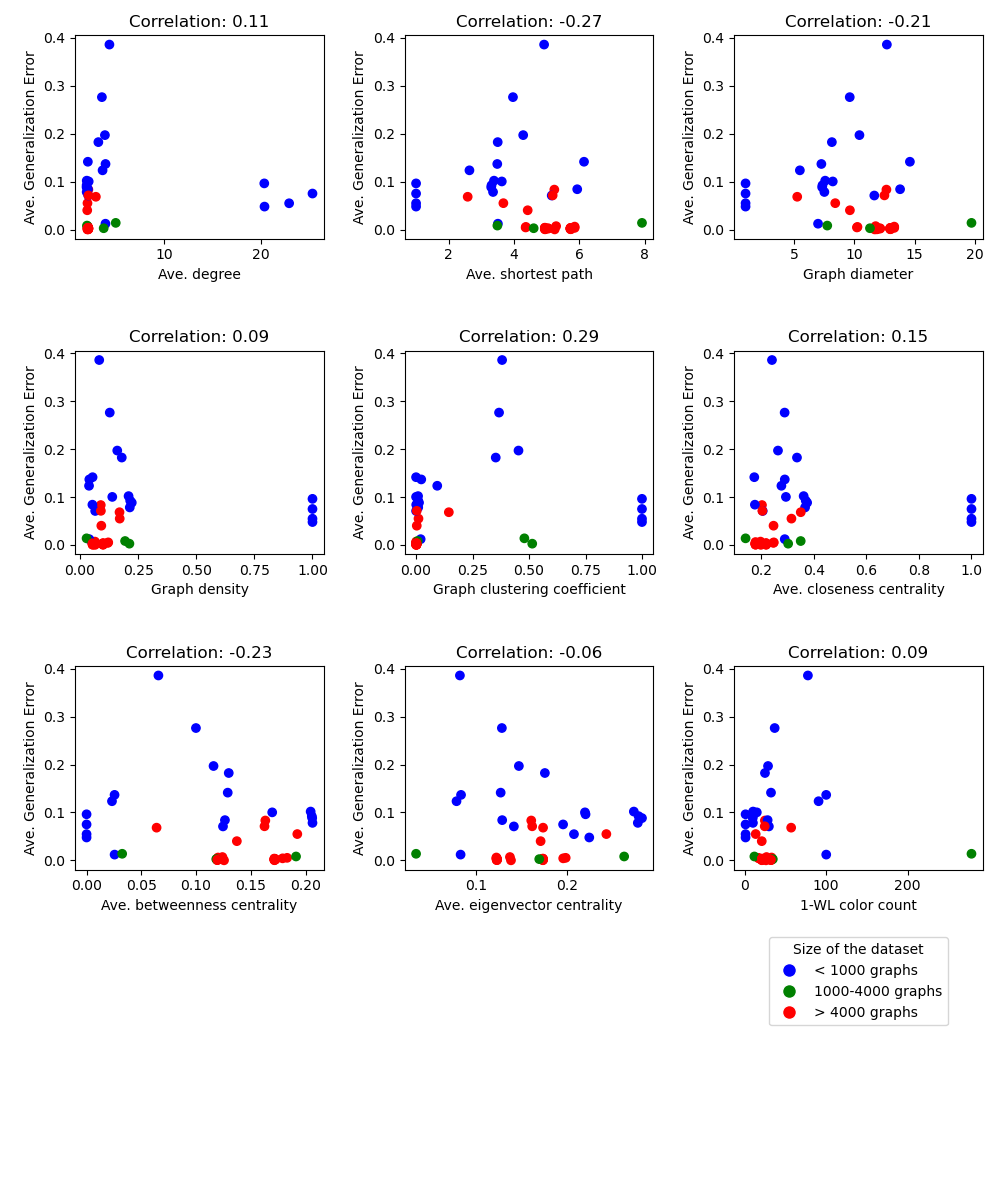
\includegraphics[scale=0.6]{images/correlation_GCN.png}
    \caption{Scatter plots showing the relationship between various graph parameters and the average generalization error of a Graph Convolutional Network (GCN). Each subplot presents the correlation coefficient between a specific graph property and the generalization error. Colors indicate dataset sizes: blue (<1000 graphs), red (1000-4000 graphs), and green (>4000 graphs).}
    \label{fig:correlation_GCN}
\end{figure}

\begin{figure}[H]
    \centering
    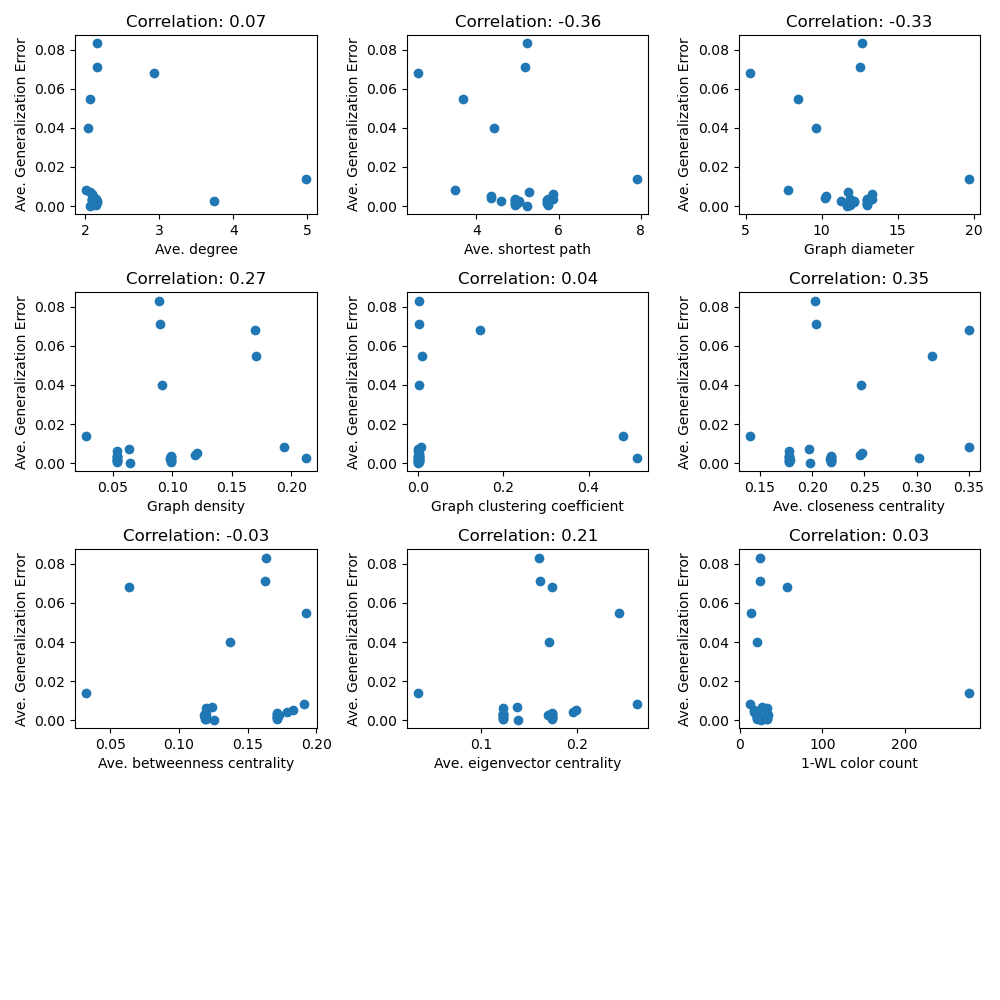
\includegraphics[scale=0.6]{images/correlation_ignore_less_than_1000_GCN.png}
    \caption{Scatter plots showing the relationship between various graph parameters and the average generalization error of a Graph Convolutional Network (GCN). Each subplot presents the correlation coefficient between a specific graph property and the generalization error. Only datasets with more than 1000 graphs are considered.}
    \label{fig:correlation_ignore_less_than_1000_GCN}
\end{figure}

\subsection{Discussion} 




\section{Simplified Graph Convolution}
The calculated generalization error of the experiments using Simplified Graph Convolution are shown in Table~\ref{tab:ge_sgc}.


\begin{table}[!ht]
    \centering
    \footnotesize
    \begin{tabular}{p{3.5cm}|p{5cm}p{5cm}}
    \hline
    \toprule
        Name & Ave. generalization error & Standard deviation \\ 
    \midrule
        AIDS & 0.0094999792054295 & 0.0067623262293636 \\
        BZR & 0.0398076958954334 & 0.0535244457423687 \\
        BZR\_MD & 0.1050406470894813 & 0.095137633383274 \\
        COLORS-3 & 0.0739687532186508 & 0.0297187566757202 \\
        COX2 & 0.0861333459615707 & 0.0670665428042411 \\
        COX2\_MD & 0.0440740659832954 & 0.1867186874151229 \\
        DD & 0.1082454919815063 & 0.0635362416505813 \\
        DHFR & 0.1035643592476844 & 0.0682980865240097 \\
        DHFR\_MD & 0.0555799715220928 & 0.1178753077983856 \\
        ENZYMES & 0.1837499886751175 & 0.0857001841068267 \\
        ER\_MD & 0.0475622005760669 & 0.0829107165336608 \\
        FRANKENSTEIN & 0.061875008046627 & 0.0329361073672771 \\
        KKI & 0.0291044823825359 & 0.2818436622619629 \\
        MCF-7 & 0.000656247138977 & 0.0137401102110743 \\
        MCF-7H & 0.001156234764494 & 0.0151891019195318 \\
        MOLT-4 & 0.0018124937778338 & 0.0116189513355493 \\
        MOLT-4H & 0.0018437386024743 & 0.0139454510062932 \\
        MUTAG & 0.1163011640310287 & 0.0678915232419967 \\
        Mutagenicity & 0.0481875017285347 & 0.0258940625935792 \\
        NCI-H23 & 0.0031250119209289 & 0.0100476266816258 \\
        NCI-H23H & 5.9604645663569045e-09 & 0.0108693270012736 \\
        NCI1 & 0.0839374884963035 & 0.0166628845036029 \\
        NCI109 & 0.0677187517285347 & 0.0309047140181064 \\
        OHSU & 0.0270329676568508 & 0.2689114809036255 \\
        OVCAR-8 & 0.0021875083912163 & 0.0154096204787492 \\
        OVCAR-8H & 0.0021250010468065 & 0.0172242671251297 \\
        P388 & 0.0042812586762011 & 0.0127577884122729 \\
        P388H & 0.0118749979883432 & 0.0183747168630361 \\
        PC-3 & -0.0001562476099934 & 0.0097229816019535 \\
        PC-3H & 0.000968748354353 & 0.0120369335636496 \\
        PROTEINS\_full & 0.0114296078681945 & 0.0617067217826843 \\
        PTC\_FM & 0.101800300180912 & 0.1584279388189315 \\
        PTC\_FR & 0.102684274315834 & 0.0604767650365829 \\
        PTC\_MM & 0.1027272716164588 & 0.1311521083116531 \\
        PTC\_MR & 0.1173060312867164 & 0.1128198280930519 \\
        Peking\_1 & 0.232065200805664 & 0.290688544511795 \\
        SF-295 & 0.0006874978425912 & 0.0154270688071846 \\
        SF-295H & 0.0021562576293945 & 0.0088528767228126 \\
        SN12C & 0.001562523888424 & 0.0126561466604471 \\
        SN12CH & -6.249547004699707e-05 & 0.0126207722350955 \\
        SW-620 & 0.0008437514188699 & 0.0120212435722351 \\
        SW-620H & 0.0024687468539923 & 0.0140694072470068 \\
        SYNTHETIC & 0.0154166761785745 & 0.0234100967645645 \\
        SYNTHETICnew & 0.1204166635870933 & 0.0984339192509651 \\
        Synthie & 0.1784375011920929 & 0.0635749474167823 \\
        UACC257 & 3.124475551885553e-05 & 0.0105321435257792 \\
        UACC257H & 5.9604645663569045e-09 & 0.0123304584994912 \\
        Yeast & 0.0027187527157366 & 0.0283915027976036 \\
        YeastH & 0.0021875023376196 & 0.0149637833237648 \\
    \end{tabular}
    \caption{Generalization error of the SGC model on 49 datasets}
    \label{tab:ge_sgc} % ge -> generalization error
\end{table}

The correlation between the generalization error and the graph parameters are shown in Figure~\ref{fig:correlation_SGC} and Figure~\ref{fig:correlation_ignore_less_than_1000_SGC}.

\begin{figure}[H]
    \centering
    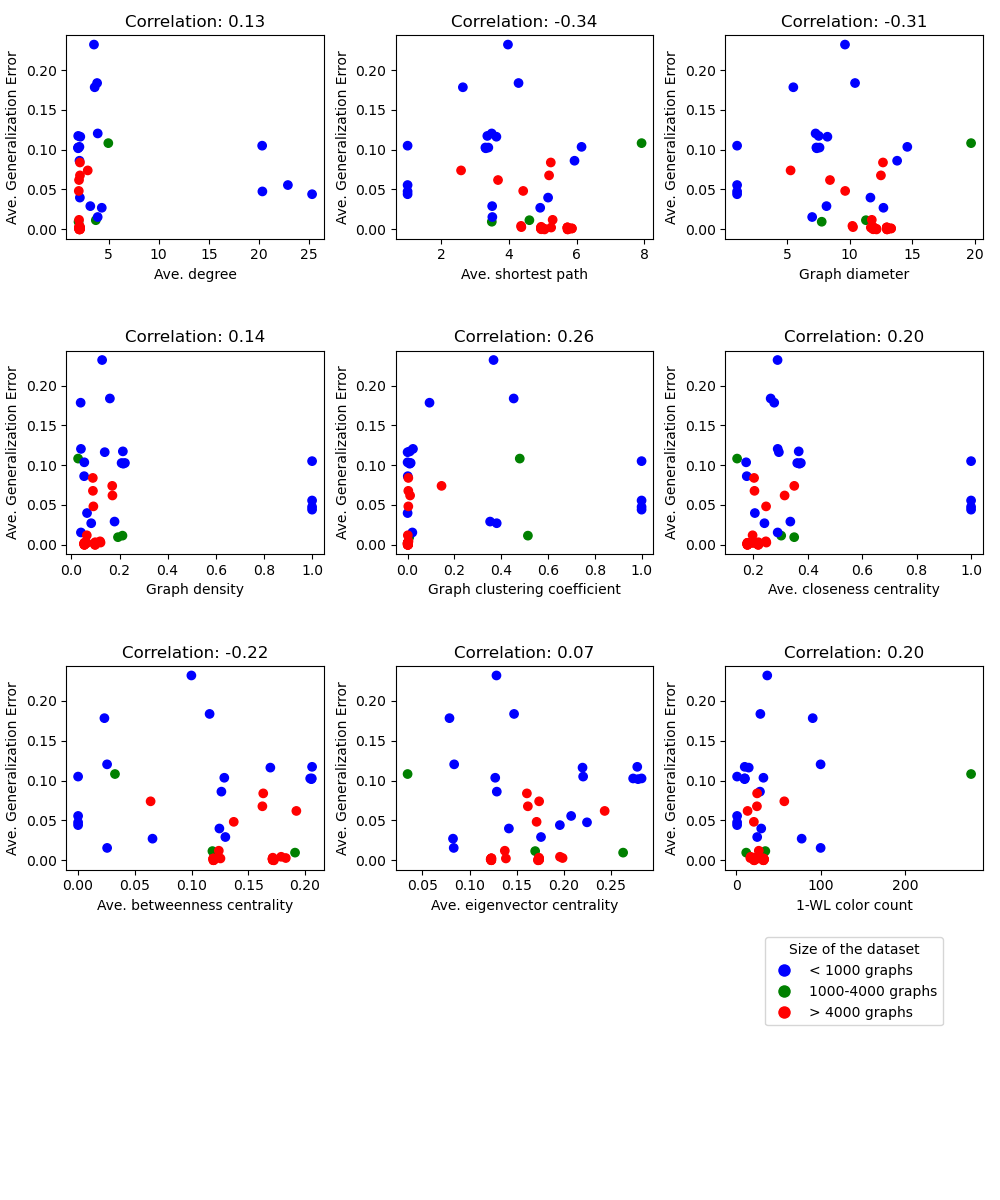
\includegraphics[scale=0.6]{images/correlation_SGC.png}
    \caption{Scatter plots showing the relationship between various graph parameters and the average generalization error of a Simplified Graph Convolution (SGC) model. Each subplot presents the correlation coefficient between a specific graph property and the generalization error. Colors indicate dataset sizes: blue (<1000 graphs), red (1000-4000 graphs), and green (>4000 graphs).}
    \label{fig:correlation_SGC}
\end{figure}

\begin{figure}[H]
    \centering
    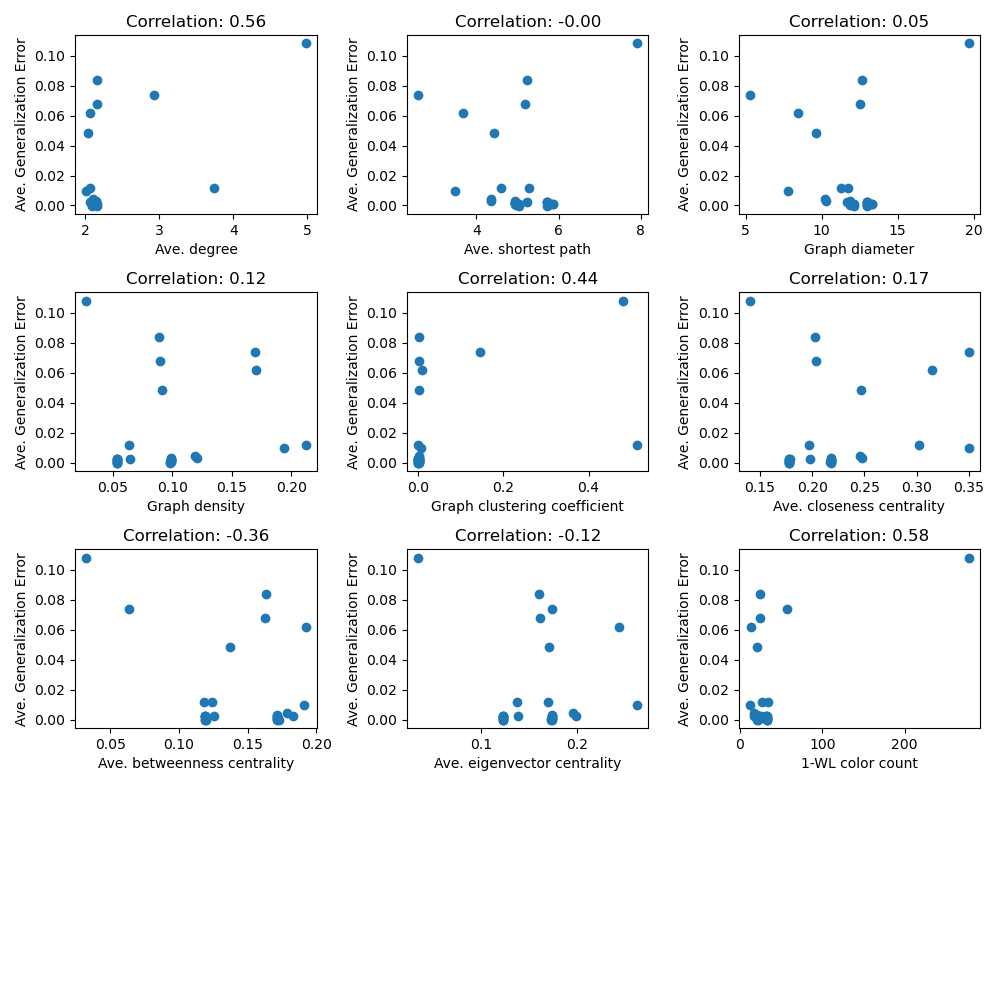
\includegraphics[scale=0.6]{images/correlation_ignore_less_than_1000_SGC.png}
    \caption{Scatter plots showing the relationship between various graph parameters and the average generalization error of a Simplified Graph Convolution (SGC) model. Each subplot presents the correlation coefficient between a specific graph property and the generalization error. Only datasets with more than 1000 graphs are considered.}
    \label{fig:correlation_ignore_less_than_1000_SGC}
\end{figure}